The lolly machine was originally constructed in the late 90's by an external company \cite{computerControlGCole}. When the machine arrived on the campus of Murdoch University, it was noted that a fundamental design criteria was completely overlooked - the machine was ordered without a control system. Fortunately Dr Graeme Cole was on the scene was able to quickly assemble and program a microprocessor based embedded system that would remain the backbone bone of the control system for decades to come. 

The lolly machine is a demonstration unit for Murdoch University Engineering that sorts and dispenses Lollies as according to their colour. The intended purpose of the lolly machine is to spark the interest of future engineering students during open days and to showcase the capabilities of Murdoch Engineering \acrlong{icse} students.

The lolly machine has been out of service for some time and is in desperate need of maintenance and an upgrade. As this is the second thesis aimed at upgrading the machine, the project has been affectionately named, \textbf{\acrfull{lmu}}.

\section{Objectives}
   This thesis project (\acrfull{lmu}) is a requirement for the Bachelor of Engineering Honours degree at Murdoch University and is worth a total of 12 credit points. ENG470 is the unit name.
   
   This thesis  has four fundamental objectives which are outlined in the following sections.
   
    
    \subsection{Objective 1: Redesign System Architecture}
        One of the main objectives of the \acrshort{lmu} is to upgrade the control system to something that is more inline with today's industrial technologies. The main intent being that future students will be able to  "play" around with the machine using technologies that are relevant with industry standards. To upgrade the control system the system architecture must be redesigned to allow the implementation of new hardware, software and communication protocols. Objective 1 is detailed in Chapter \ref{chap:sysArch}
        
    \subsection{Objective 2: Develop Machine Program}
        With the installation of new control system hardware comes the task of developing new code to suit.
        Objective 1 captures all aspects of program development in regards to the \acrshort{plc}, such items include.
        \begin{itemize}
            \item \acrshort{io} mapping
            \item Program design using various techniques
            \item Develop "special" functions
        \end{itemize}

        
        
    \subsection{Objective 3: Develop HMIs}
        
        One of the objectives from the previous thesis project was to \textit{"Develop a NI LabVIEW status display program to allow user interaction via a PC"} \cite{thesisJodie}. The essence of this previously defined objective has been taken onboard and enriched. A total of three \acrshort{hmi}s have been developed for the lolly machine. All of which have the ability to control and monitor the status of the machine. \acrshort{hmi}s include a Siemens touch panel which is physically mounted to the machine, a LabVIEW program that can be installed as a run-time application on any computer that is connected to the machine and a web based application which has been built on a Raspberry-Pi microcontroller.
        
    \subsection{Objective 4: Create User Documentation}
        The final objective was to create documentation so that the users are able to operate and troubleshoot the machine. Documents include:

        \begin{enumerate}
            \item   User Manual
            \item   Electrical Drawings
            \item   Modbus Register
            \item   \acrshort{io} List
            \item   \acrshort{plc} program
            \item   \acrshort{hmi} program
            \item   LabVIEW program
            \item   Node-RED program
        \end{enumerate}
        
        User documentation is attached within the appendix of this document


    % REPLACE WITH NEW PHOTO OF NEW INSTALL
    \begin{figure}[ht]
        \centering
        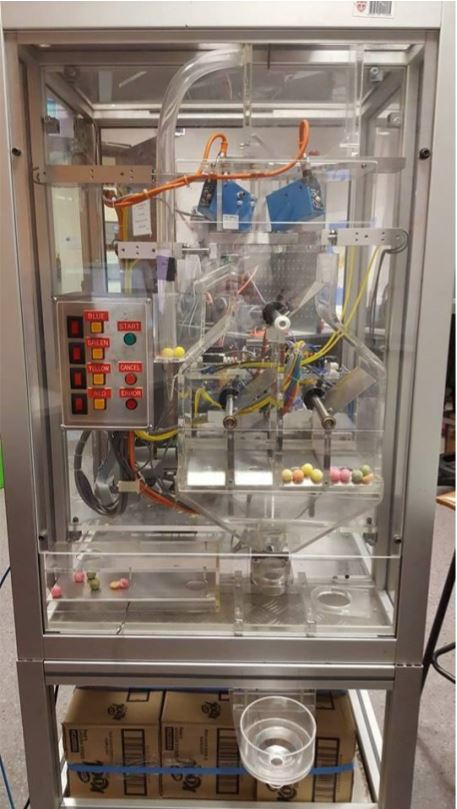
\includegraphics[scale = 0.5]{lollyMachine.JPG}
        \caption{The lolly machine~\cite{thesisJodie}.}
        \label{fig:lollyMachine}
    \end{figure}
